%!TEX root = ../thesis.tex
%Adding the above line, with the name of your base .tex file (in this case "thesis.tex") will allow you to compile the whole thesis even when working inside one of the chapter tex files

\chapter{Data Analysis} \label{chap:4}

The complex visibilities outputted from the correlator of a radio interferometer are far from ideal and many additional steps of processing are required before they can be of scientific use. The imperfection of the synthesis radio telescopes (e.g., surface accuracy, receiver noise, gain stability, etc.), the adjustments to the signal (e.g., filter bandpass, etc.), hardware or software failures, poor atmospheric conditions, and the presence of RFI are some of the many sources of visibility corruption that must be accounted for before they can be Fourrier transformed to get the sky brightness distribution. This chapter describes the three main steps involved in reducing any standard radio interferometric data set, namely: data examination and flagging, data calibration, and imaging. In each step we give relevant examples of the data reduction techniques used in \cite{ogorman_2012} and \cite{ogorman_2013}. A general work flow chart is given in Figure \ref{fig:4.1} which highlights the standard procedure required to go from raw visibilities to image analysis and summarizes what will be discussed in this chapter.\\
\\
\begin{figure}[hbt!]
\centering 
          \includegraphics[trim=20pt 270pt 0pt 230pt,clip,scale=0.8]{/home/eamon/thesis/thesis_template/4/cash_flow.ps}
\caption[Radio interferometry work flow chart]{Work flow chart highlighting the general procedure required to go from the raw visibilities outputted by the correlator to a final radio image that can be used for scientific analysis. (Image adapted from the CASA cookbook, NRAO)}
\label{fig:4.1}
\end{figure}

\section{Data Examination and Flagging}\label{sec:4.1}
The Common Astronomy Software Application \citep[CASA;][]{mcmullin_2007} package was used to flag, calibrate, and image the main data sets used in this thesis. CASA is operated through a Python interface and uses a suite of astronomical data reduction tools which have been developed to meet the processing requirements of the large  data sets from the Karl G. Jansky VLA and ALMA. It can also be used to process data from practically all other modern radio synthesis arrays. For synthesis data to be processed in CASA, it must be in a ``measurement set'' format. VLA data is easily transferable into this format using the \textit{importevla} task within CASA. CARMA data files however come in \textit{Miriad} format and need to be first converted into Flexible Image Transport System (i.e., FITS) format within the Miriad \citep{sault_1995} data reduction package. During this process the raw data are smoothed by a Hanning filter (combining adjacent frequency channels with weights 0.25, 0.5, and 0.25) to dampen ringing in the bandpass. Once in FITS format, the data can then be imported into CASA using the \textit{importuvfits} task.

Once the data has successfully been imported into CASA the \textit{listobs} task can be used to get a summary of the data set allowing the user to make sure the observing track contains the requested sources at the correct times. At this point it is also a good idea to check any observing logs which are created on site during the observation by the array operators. These logs usually contain important information about the specific track such as non-operational antennas, unavailable receivers, weather conditions etc., and such data will need to be treated appropriately during calibration or flagged at this stage. The \textit{plotms} task, which is a GUI-style plotter, can then be used to obtain X-Y plots of visibility data. A good visual overview of the observation track is obtained by plotting all the source visibility amplitudes as a function of time. Averaging the data over channels or baselines often alerts the user of obvious bad data, which can be manually flagged through the \textit{plotms} interface or through the \textit{flagdata} task. An example of such a plot is shown in Figure \ref{fig:4.2} where the visibility amplitudes of three sources in a 1.3\,cm VLA observing track for Aldebaran are displayed against time. The relatively weak target is shown between interleaving scans of the stronger phase calibrator, while the flux calibrator is the scan at the end of the observing track and is the strongest source in this observation. The data has been averaged over all channels and over a time period of x\,s. Some relatively low visibility amplitudes can clearly be seen for all scans of the phase calibrator which can be traced to a single poor performing antenna.

\begin{figure}[hbt!]
\centering 
\includegraphics[trim=20pt 240pt 0pt 230pt,clip,scale=0.75]{/home/eamon/thesis/thesis_template/4/c_overview.ps}  
\caption[Data examination of a VLA data set.]{Data examination of a 6\,cm VLA data set for Aldebaran. A good visual overview of the observation track is obtained by plotting all the source visibility amplitudes as a function of time. Averaging the data over channels or baselines sometimes allows rogue data to stand out. Here the black, orange, and green data points represent the phase calibrator, the science source, and the flux calibrator. The left most black data points are part of the dummy scan which has to be flagged. The low data points of the phase calibrator are data which needs further investigation. The absence of data at certain times is just when observations at 3\,cm where being taken.}
\label{fig:4.2}
\end{figure}

Another important way to represent the data at this stage of the flagging process is to plot the visibility amplitude of each of the sources as a function of $u-v$ distance or baseline length (i.e., $\sqrt{(u^2 + v^2)}$). The amplitude distribution should be relatively constant as a function of $u-v$ distance for the phase calibrator (i.e., a point source) and will fall off with increasing baseline length if the flux calibrator is resolved. Plotting the data in this format often results in extreme points at certain baselines which can then often be traced back to poorly behaving antennas or baselines. There is also some flagging which can be carried out based in part on a priori information. Antennas in very compact configurations can partially block the incoming RF signal to other antennas which is often referred to as antenna shadowing. This was not a problem in our VLA B configuration observations but some data obtained in the more compact CARMA configurations had to be flagged as a result of this shadowing. At the time our VLA observations took place, every observing track (i.e., scheduling block) needed to commence with at least a one minute \textit{dummy scan} to facilitate the correlator setup. We subsequently flagged these scans as they contained no useful scientific data. Other a priori flagging was to remove any visibilities with zero amplitudes and to flag the edge channels in the CARMA data sets. Finally visual inspection of each scan was carried out to determine if data at the beginning or end of these scans needed to be flagged. This processes is often referred to as quacking in radio interferometry analysis.

No RFI was present in any of the CARMA data sets and in any of the VLA data sets at wavelengths $\lesssim 3$\,cm (i.e., X, K, Ka, and Q bands). For the 2011 long wavelength ($> 3$\,cm) data the two sub-bands were centered at relatively RFI free regions of the bandpass and only a very small amount of RFI had to be manually flagged. The 2012 wide-band data was taken at 10\,cm (i.e., S band) and 20\,cm (i.e., L band) and many of the sub-band were severely contained with RFI especially at 20\,cm. In Figure \ref{fig:4.3} we plot the visibility amplitude of the flux calibrator 3C286 against frequency for the 2012 wide-band data set at 20\,cm. The upper panel shows the raw data before any RFI has been removed. Some of the sub-bands were so contaminated with RFI that they had to be completely flagged. The remaining sub-bands were initially Hanning smoothed to suppress Gibbs ringing. This action spreads the single-channel RFI into three channels, but importantly removes the effects of some of the worst RFI from a number of channels and allows as much good data to be retained as possible. The \textit{testautoflag} task was then used to conservatively flag RFI from all sources and any remaining RFI was manually flagged. The final result for the flux calibrator is shown in the bottom panel of Figure \ref{fig:4.3} with only some residual RFI still remaining, particularly between 1 and 1.2\,GHz.

\begin{figure}[hbt!]
\centering 
\includegraphics[trim=30pt 70pt 20pt 70pt,clip,width=14cm,height=14cm]{/home/eamon/thesis/thesis_template/4/rfi_thesis_new.ps}  
\caption[Eliminating RFI from the L band data set.]{Eliminating RFI from the 20\,cm wide-band data set. \textit{Top panel:} Raw visibility amplitudes showing the presence of high levels of RFI in many sub-bands. \textit{Bottom panel:} Post flagging visibility amplitudes. Some of the sub-bands were so severely contaminated with RFI that they had to be completely flagged. The data is still uncalibrated at this stage and the gain as a function of frequency is clearly present.}
\label{fig:4.3}
\end{figure}

\section{Calibration}\label{sec:4.2}

The role of calibration is to correct the measured visibilities $V'(u,v)$ to approximate as closely as possible the true visibilities $V(u,v)$. As discussed in Chapter \ref{chap:2}, the true visibilities are related to the sky brightness via the Fourier transform:
\begin{equation}
V_{ij}(t) = \int A(l,m) I(l,m) \mathrm{exp}[-i2\pi(u_{ij}(t)l + v_{ij}(t)m)]	dl	dm
\end{equation}
where $i,j$ represent the discrete sampling of the antennas $i$ and $j$ at time $t$. The term $u_{ij}(t)l + v_{ij}(t)m$ is the geometric phase difference produced by the geometric path length difference between antenna $i$ and antenna $j$ from the source (or part of) at location ($l,m$) relative to the phase center. The relationship between the measured visibility and the true visibility on a baseline between antennas $i$ and $j$ may be expressed as
\begin{equation}
V_{ij}' =  J_{ij}V_{ij}
\end{equation}
where $ J_{ij}$ represents the accumulation of all corruptions affecting baseline $ij$. This equation is known as the Hamaker-Bregman-Sault Measurement Equation \citep{hamaker_1996}. The most important of the effects contained in $J_{ij}$ are antenna-based and arise from the measurable physical properties of individual antenna elements or the measurable physical conditions in the atmosphere above them. Thus, an array of $N$ antennas forming $N(N-1)/2$ baselines can usually be adequately calibrated through the determination of only $N$ factors.

For the purpose of the work presented in this thesis, the Measurement Equation can be written as
\begin{equation}
V_{ij}'(u,v,\nu) = b_{ij}(t)[B_{i}(\nu ,t)B_{j}^{*}(\nu ,t)](t)g_{i}(t)g_{j}(t)V_{ij}(u,v,\nu)e^{i[\theta _{i}(t) - \theta _{j}(t)]}
\end{equation}
where
\begin{itemize}
\item $g_{i}$ and $\theta _{i}$ are the amplitude and phase portions of the complex gain which are usually determined separately in the calibration process and may change over the observation period with temperature, atmospheric conditions, etc. 
\item $B_{i}$ is the complex bandpass, the instrumental response as a function of frequency, $\nu$ and may also vary over time.
\item $b_{ij}(t)$ is the baseline term and is important shortly after a configuration change when antenna positions may not be known well.
\end{itemize}
The general calibration strategy is then to derive a series of scaling factors from both the phase and flux calibrators, which are then collectively applied to the science target in the final stage of calibration. A general workflow diagram describing the main steps involved in calibration process are summarized in Figure \ref{fig:4.3}. We now discuss each of these steps while placing emphases on our CARMA and VLA data.

\begin{figure}[hbt!]
\centering 
\includegraphics[trim=20pt 160pt 0pt 140pt,clip,scale=0.6]{/home/eamon/thesis/thesis_template/4/calib_overview.ps}  
\caption[Calibration workflow diagram.]{A workflow diagram outlining the main steps involved in calibrating radio interferometric data. Each of these steps are discussed in the text in relation to our CARMA and VLA observations.}
\label{fig:4.3}
\end{figure}

\subsection{Prior Calibration}
Our 2011 VLA data were acquired just after an array re-configuration which meant that the positions of some of the antennas were not accurately known at the time of observations. This resulted in some data points having inaccurate $u-v$ coordinates. During the course of observations in each configuration, the exact position of all antennas become known and so the $u-v$ data could be calibrated to account for the discrepancies in the $u-v$ coordinates.  At the VLA site, atmospheric opacites become significant at frequencies $\gtrsim 20$\,GHz as shown in Figure \ref{fig:4.3}. Therefore, atmospheric opacity corrections were applied to the high frequency data sets. The adjustment values were based on the average of a seasonal model (based on many years of measurements) and information from the weather station obtained during the observations. For the CARMA data, the opacity at 1.3\,mm is measured by a tipper \citep{white_2009}. The tipper reflects radiation from the blank sky at different inclination onto a radiometer. The voltage from the radiometer can then be plotted against inclination to allow the opacity to be calculated. 

The final a priori calibration step is to provide a flux density value to the flux calibrator via CASA's \textit{setjy} task. The VLA flux calibrators were assigned values using the ``Perley-Butler 2010" flux density standard models  and with assumed systematic uncertainties of 3\% at all frequencies \citep{perley_2013}. At the time, no Ka or S-band flux density standard models were available so instead for these we used the K and L-band models, respectively, which were scaled according to their spectral indices. The absolute flux scale for CARMA observations is often determined by observing a planet and using a model of its flux as a function of baseline length. However, no such models were available in the early version of CASA and so the flux calibration was carried out with the quasers, 0530+135 and 3C120. The continuously updated CARMA flux catalog was accessed via the \textit{xplore} GUI to obtain their flux values at each observation. The flux of these objects are more unpredictable and the systematic uncertainties are about 20\%.

\begin{figure}[hbt!]
\centering 
\includegraphics[trim=20pt 320pt 0pt 300pt,clip,scale=0.7]{/home/eamon/thesis/thesis_template/4/opacity.ps}  
\caption[Atmospheric opacity at the VLA site.]{Calculation of the atmospheric opacity at the VLA site between $1-50$\,GHz on 2011 February 11. The adjustment values applied to the data were based on the average of a seasonal model and information from the weather station obtained during the observations.}
\label{fig:4.4}
\end{figure}

\subsection{Bandpass Calibration}
The bandpass is the relative gain as a function of frequency and solving for it is the first part of the calibration process. Variation in frequency arises from frequency dependent effects in signal transmission. Such variation is shown in Figure \ref{fig:4.5} for both phase and amplitude for a single antenna. For the VLA data, the flux calibrators were also used as the bandpass calibrators. Their phases were found to vary significantly over the $5-10$ minutes of observation especially at high frequencies; in most cases by a few 10s of degrees. Before a solution to the bandpass could be found, these phase variations needed to be corrected for to prevent decorrelation of the vector averaged bandpass solution. The complex bandpass, $B_i$ could then be solved using the \textit{bandpass} task and applying the antenna positions and phase solutions. The bandpass solutions  were then applied to the bandpass calibrator to make sure both the amplitude and phase were then almost constant across channels/frequency.

\begin{figure}[hbt!]
\centering 
\includegraphics[trim=20pt 320pt 0pt 300pt,clip,scale=0.77]{/home/eamon/thesis/thesis_template/4/bandpass.ps}  
\caption[Gain variation as a function of frequency.]{One antenna's gain variation as a function of frequency for the flux calibrator 3C138 at 1.3\,cm. Bandpass calibration corrects for this variation.}
\label{fig:4.5}
\end{figure}

The CARMA data contained three spectral windows (i.e., 468, 62, and 31\,MHz in width), each having independent bandpass shapes in both amplitude and phase. For each of these spectral windows, the gain calibrations are typically the same  after the full bandpass dependence has been removed. The strategy to calibrate the CARMA data was to initially carry out the bandpass calibration on the wideband data (i.e., 468\,MHz) using the same strategy outlined in the previous paragraph and then carry out the gain calibration on this wideband data. Once this had been done, these bandpass independent gain solutions were applied to the narrow band data (i.e., 62, and 31\,MHz) while solving for their bandpass. This narrow band bandpass solution could then be applied to the target and phase calibrator.

\subsection{Gain Calibration}

Once a bandpass solution has been applied, the next step is to derive corrections for the antenna amplitude and phase gains, $g_{i}$ and $\theta _{i}$, as a function of time. In order to determine the appropriate antenna-based complex gains for the science target, a phase calibrator which is always a point source and located much closer to the target than the flux calibrator, is regularly observed to minimize differences through the atmosphere. The general procedure then is to solve for these antenna-based gain factors for each scan on all calibrators. The amplitude changes on a much longer timescale than the phase and so they are solved separately. If there is a substantial change in phase over a scan and the un-corrected phases were averaged over this timescale, then the amplitude would be decorrelated. It is therefore important to correctly determine appropriate scan lengths when preparing the observations, especially at high frequencies, where  time-dependent gain errors are introduced by the troposphere.

During gain calibration, the relative gain amplitudes and phases for different antennas are determined using the phase calibrator. The \textit{gaincal} task is used to do this. The absolute flux density scale of the phase calibrator is later determined by comparison against the gain amplitudes $g_{i}$ derived for the flux calibrator. To find the relative phases, a zero phase is determined by selecting a reference antenna for which the phase is defined to be zero. In the first step new solutions of complex gains $g_{i}$ and $\theta _{i}$ are derived for the flux density calibrator which are corrected for the bandpass shape (here we assume the flux density calibrator has been used as the bandpass calibrator as was the case for our observations). The second and final step requires the determination of the appropriate complex gains from the phase calibrator.

\subsection{Flux Scale Calibration and Application of Solutions}\label{subsec:2.4}
The penultimate stage of the calibration process is to use the known flux density of our flux calibrator (whose flux density was set using \textit{setjy} above) to derive the flux density of the phase calibrator, which was previously assumed to be a point source of 1\,Jy located at the phase center. This is achieved using the \textit{fluxscale} task. The final step of the calibration process is to apply the calibration solutions to the actual data, using the task \textit{applycal}. During this process, the calibration solutions are applied to the DATA column in the measurement set, and the results are written in the CORRECTED$\_$DATA column of the measurement set. For the calibrators, the phase and amplitude calibration comes from their own solutions and the bandpass solutions come from the bandpass calibrator. For the science target we again apply the bandpass solution from the bandpass calibrator but the gain solutions come from the close by phase calibrator. Once calibration of the data is complete, it is worth spending time inspecting the corrected data to make sure there are no obvious errors in the data. If such errors are indeed found at this stage, then their cause will need to be flagged and the data must be re-calibrated. Some insightful plots to investigate how successful the calibration was, are: amplitude vs time, amplitude vs $u-v$ distance, and amplitude vs phase. If a point source has being successfully calibrated then it will have an appearance similar to that in Figure \ref{fig:4.6}, i.e., a compact ball of visibilities centered at zero phase and at the amplitude found for that source. 

\begin{figure}[hbt!]
\centering 
\includegraphics[trim=20pt 240pt 0pt 220pt,clip,scale=0.77]{/home/eamon/thesis/thesis_template/4/calib_x_phase_amp.ps}  
\caption[Example of a well calibrated source.]{A well calibrated source will produce a compact ball of visibilities centered at zero phase and at the amplitude found for that source. Here we plot the calibrated visibilities at 3\,cm for J0449+1121; the phase calibrator in the 3\,cm data set for Aldebaran.}
\label{fig:4.6}
\end{figure}

\section{Imaging}\label{sec:4.3}

% evla paper

%The image cubes were multiscale CLEANed down to the
%3 threshold using natural weighting and were corrected for
%primary beam attenuation. The multiscale algorithm (Rich et al.
%2008) within CASA was set to four unique scales; the largest
%corresponding to the largest structures visible in individual
%channel maps. Each scale was approximately set to three times
%smaller than the preceding scale.
%
%The visibilities were then both Fourier transformed and deconvolved using the CASA \textit{clean} task in multi-frequency synthesis imaging mode, which separately grids the multiple spectral channels onto the \textit{u-v} plane and therefore improves the overall \textit{u-v} coverage. We used natural weighting for maximum sensitivity and the cell size was chosen so that the synthesized beam was about five pixels across. For the high frequencies it was usually sufficient to place just one CLEAN circle around the target source.  For the low frequencies however, the image sizes were usually set to a few times the size of the primary beam so that nearby strong serendipitous sources could be CLEANed thus reducing their sidelobe contamination of the final image. These images were CLEANed interactively, taking sky curvature into account, down to about the $3\sigma$  level with clean boxes placed around sources as they appeared in the residual image. All images were corrected for  primary beam attenuation. 
%
%CLEAN vs MEM vs Multi-scale Clean (for Peter!)
%
%second sources (maps)
%
%Dirty Image, PSF
%
%Show images of calibrators